\documentclass[10pt,twocolumn,letterpaper]{article}
\usepackage[margin=0.7in,columnsep=0.25in]{geometry}
\usepackage{amsmath,amssymb,graphicx,booktabs,caption}
\makeatletter\newcommand\tabinput[1]{\@@input #1 }\makeatother
\usepackage[numbers,sort&compress]{natbib}
\captionsetup{font=small,labelfont=bf}
\setlength{\parskip}{0pt}
\makeatletter\renewcommand\section{\@startsection{section}{1}{0pt}{-7pt}{2pt}{\normalfont\large\bfseries}}\makeatother
\title{\vspace{-0.6in}\Large A relativistic check of the CoE toy model: the nearby Hubble anisotropy, with the CMB as an open issue}
\author{Note for Chris, \today}
\date{\vspace{-0.35in}}
\begin{document}
\maketitle

\begin{abstract}\noindent
Your toy model has a real centre of expansion (CoE), gravity as the only force, an always-decelerating expansion and no dark matter, and it is built to explain the Migkas cluster anisotropy. Because the enclosed mass has $2GM/c^2>D$, we recompute it with an exact Lema\^itre--Tolman--Bondi dust model. General relativity confirms the Newtonian result. The anisotropy is almost pure $m=2$, it is aligned with the CoE axis, and with the corrected sign $A\propto H_0^2$ its maximum lies on the axis as in the data. The shell theorem shows why only the net mass inside $D-R$ matters and why it must be positive. We also trace the CMB through the same pure-dust model. Without further physics the stretch to last scattering is not isotropic, and we record this as an open issue for a later stage. The observed CMB dipole is kinematic and is not needed to support the model.
\end{abstract}

\section{Question}
The Migkas et al.\ \cite{Migkas2020,Migkas2021} cluster anisotropy is a direction dependence of the local expansion rate at $z\lesssim0.3$. Your toy model explains it with the tidal field of a large mass toward the CoE, with gravity as the only force and no accelerated expansion. The CoE mass is unlabelled gravitating mass, and the model contains no dark matter. Your integration is Newtonian (Table~\ref{tab:vars}), while $2GM/c^2>D$, so we ask whether the same geometry gives the same nearby pattern in general relativity. We also report what the pure-dust version gives for the CMB, as input for a later stage.


\begin{table}[h]\centering\footnotesize
\caption{Your variables and the best fit being tested. $M_{\rm crit}=H_0^2D^3/2G$ is the critical mass inside $D$.}\label{tab:vars}
\begin{tabular}{@{}lll@{}}\toprule
Symbol & Meaning & Value\\\midrule
$D$ & Earth--CoE distance today & 41.53 Gpc\\
$L$ & scale of the $e^{-r/L}$ density & 2.919 Gpc\\
$M$ & mass inside $D$ & $1.944\times10^{54}$ kg\\
$M/M_{\rm crit}$ & & 0.0239\\
$R$ & vision-shell radius & 14.3 Gpc\\
$\ell_0$ & anti-CoE longitude ($b=0$) & $13.2^\circ$\\
$\ell_0+180^\circ$ & CoE longitude & $193.2^\circ$\\
$H_0$ & local expansion rate [km/s/Mpc] & 70\\
$k$ & Newtonian rate [s$^{-1}$], $t_0=1/k$ & $2.18\times10^{-18}$\\
$2GM/(c^2D)$ & & 2.25\\\bottomrule
\end{tabular}\end{table}


\section{Which mass matters: the shell theorem}
Let $R$ be the radius of our visible sphere, centred on Earth at distance $D$ from the CoE, and let $\bar\rho$ be a density that is uniform across the visible sphere. For matter arranged spherically about the CoE, the field inside the visible sphere is
\begin{equation}\label{eq:shell}
\mathbf g(\mathbf x)=-\frac{GM_{\rm net}\,\mathbf y}{|\mathbf y|^{3}}-\frac{4\pi G\bar\rho}{3}\,\mathbf y,\qquad \mathbf y=\mathbf x-\mathbf x_{\rm CoE},
\end{equation}
\begin{equation}\label{eq:mnet}
M_{\rm net}=M(<D-R)-\tfrac{4\pi}{3}\bar\rho\,(D-R)^3 .
\end{equation}
Any spherically symmetric distribution inside $D-R$ acts as a point at the CoE. A uniform shell that contains the visible sphere adds only the second term of Eq.~(\ref{eq:shell}), which is isotropic and changes only the mean expansion rate. Symmetric matter beyond $D+R$ exerts no net pull. The anisotropy therefore comes only from the net mass inside $D-R$, which is the core minus the hole swept out of the uniform density, through the traceless tidal tensor at the observer,
\begin{equation}\label{eq:tide}
\frac{\partial g_i}{\partial x_j}\bigg|_{\rm obs}=\frac{GM_{\rm net}}{D^3}\left(3n_in_j-\delta_{ij}\right)-\frac{4\pi G\bar\rho}{3}\delta_{ij}.
\end{equation}
For $M_{\rm net}>0$ the flow is stretched along the CoE axis, so $H$ is largest on the axis. For $M_{\rm net}<0$ the $m=2$ pattern flips and $H$ is largest across the axis. In GR, Birkhoff's theorem carries the same statements over to the LTB model below, where the net mass is the mass function $M(r)$ with any uniform background removed.

\section{Dust model}
We use the Lema\^itre--Tolman--Bondi (LTB) metric \cite{Bondi1947,Bolejko2011} with $G=c=1$,
\begin{equation}\label{eq:ltb}
ds^2=-dt^2+\frac{R'^2}{1+2E(r)}\,dr^2+R^2d\Omega^2,
\end{equation}
\begin{equation}\label{eq:fried}
\dot R^2=\frac{2M(r)}{R}+2E(r),
\end{equation}
where $r$ labels comoving dust shells, $R(r,t)$ is the areal radius, a prime is $\partial_r$ and a dot is $\partial_t$. The local density is $\rho=M'/(4\pi R^2R')$. With bang time $t_B(r)$ the exact solution is
\begin{equation}\label{eq:sol}
R=M^{1/3}(t-t_B)^{2/3}g(w),\qquad w=\frac{E\,(t-t_B)^{2/3}}{M^{2/3}},
\end{equation}
where $g$ is obtained from the parametric hyperbolic and elliptic solutions (with a Taylor series for $|w|<0.15$), so that $R$, $R'$, $R''$, $\dot R$ and $\dot R'$ are analytic. The mass function is your profile,
\begin{equation}\label{eq:M}
\begin{gathered}
M(r)=M\,\frac{F(r/L)}{F(r_{\rm obs}/L)},\\ F(X)=1-e^{-X}\left(1+X+\tfrac12X^2\right),
\end{gathered}
\end{equation}
and the observer's local rate is fixed by the expansion scalar,
\begin{equation}\label{eq:H}
\tfrac13\left(H_r+2H_\perp\right)=H_0,\qquad H_r=\dot R'/R',\quad H_\perp=\dot R/R.
\end{equation}

The first construction (case A) takes $r$ as the areal radius today, $R(r,t_0)=r$, with a uniform bang time. Then $E(r)$ is fixed by the age and only $t_0$ is free, set by Eq.~(\ref{eq:H}). This case is not realisable. Across a wide range of radii the age condition demands $1+2E<0$ (Table~\ref{tab:model}), i.e.\ a shell whose maximum radius lies inside its own Schwarzschild radius, which has no dust LTB realisation \cite{Hellaby1985}. The reason is that your fixed-profile core has $2GM(r)/c^2\gg r$ at those radii, and no bound shell that stays outside $2M$ can be at $R=r$ with age $t_0$. A dust LTB cannot hold your present-day profile in place.

The second construction (case B), used for all results, puts the profile on the Lagrangian label $r$ and gives each shell the energy of your Newtonian initial condition $v=x/t$,
\begin{equation}\label{eq:E}
E(r)=\frac{r^2}{2t_0^2},\qquad t_B=0 .
\end{equation}
The observer shell $r_{\rm obs}$ and $t_0$ are fixed by $R(r_{\rm obs},t_0)=D$ and Eq.~(\ref{eq:H}), so $M$ is the mass inside areal radius $D$. $E>0$ everywhere, no shell recollapses, and $R'>0$ throughout (no shell crossing), so no bang-time gradient is needed. Because the core now expands with the flow, its density today is far below the fixed-profile value (Table~\ref{tab:model}). The expansion at the observer is anisotropic, faster along the CoE line than across it.

\begin{table}[h]\centering\footnotesize
\caption{LTB construction. Case A is your profile on today's areal radius; case B is the regular model used below.}\label{tab:model}
\begin{tabular}{@{}lr@{}}\toprule
\tabinput{tab_model.tex}\bottomrule
\end{tabular}\end{table}

\begin{figure*}[t]\centering
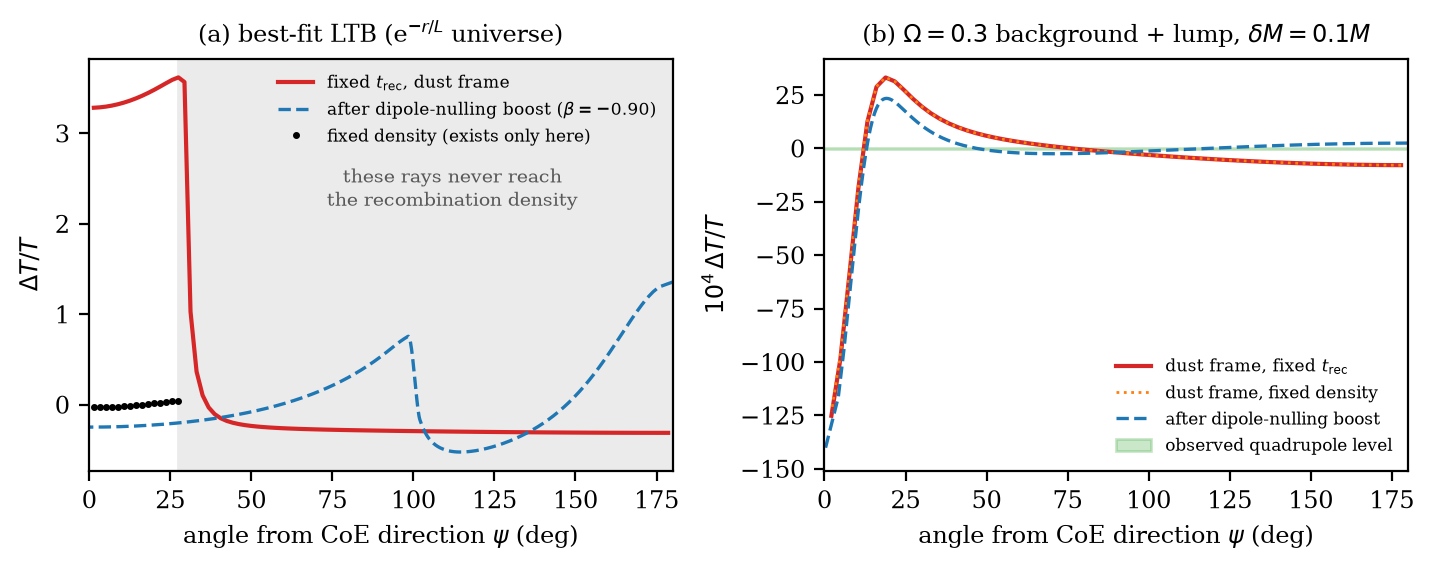
\includegraphics[width=0.74\textwidth]{fig_dT.png}
\caption{$\Delta T/T$ against the angle from the CoE. (a) Best-fit LTB (case B): definition (a) in the dust frame (red) and after the boost that removes the dipole (dashed), and definition (b) (dots), which exists only in the unshaded cap. (b) The same analysis with a homogeneous $\Omega=0.3$ background added and one tenth of the lump mass, in units of $10^{-4}$. The green band is the observed quadrupole level.}\label{fig:dT}
\end{figure*}
\begin{table*}[t]\centering\small
\caption{CMB multipoles $|c_\ell|$ of $\Delta T/T$ and the boost $\beta$ that removes the dipole. ``Scaled'' rows are the linear background-plus-lump models rescaled so that the nearby $A$ has the data's $m=2$ amplitude.}\label{tab:mult}
\setlength{\tabcolsep}{3pt}
\begin{tabular}{@{}lccccc@{}}\toprule
Model & $\beta$ & $c_1$ & $c_2$ & $c_3$ & $c_4$\\\midrule
\tabinput{tab_mult.tex}\bottomrule
\end{tabular}\end{table*}
\section{Ray tracing and last scattering}
Past null geodesics from the observer are traced in the plane containing the CoE line, following Alnes \& Amarzguioui \cite{Alnes2006} and Foreman et al.\ \cite{Foreman2010}. With affine parameter $\lambda$ and $J=R_{\rm obs}\sin\psi$ conserved,
\begin{equation}\label{eq:geo}
\begin{aligned}
\frac{dk^t}{d\lambda}&=-\frac{R'\dot R'}{1+2E}(k^r)^2-R\dot R\,\frac{J^2}{R^4},\\
\frac{dk^r}{d\lambda}&=-2\frac{\dot R'}{R'}k^tk^r-\Big(\frac{R''}{R'}-\frac{E'}{1+2E}\Big)(k^r)^2+\frac{(1+2E)J^2}{R'R^3},
\end{aligned}
\end{equation}
with $d\theta/d\lambda=J/R^2$, $k^t_0=-1$ and $k^r_0=-\cos\psi\sqrt{1+2E}/R'$, where $\psi$ is the angle between the viewing direction and the CoE. The clock $\ln(t_0/t)$ is the integration variable (DOP853, relative tolerance $10^{-12}$), and $1+z=-k^t$. The last-scattering surface (LSS) is defined as (a) a fixed proper time since the bang, $t=t_{\rm rec}$, or (b) a fixed local density, $\rho=\rho_{\rm rec}$, with $t_{\rm rec}$ or $\rho_{\rm rec}$ chosen so that the monopole is $1+\bar z=1090$. With $T\propto1/(1+z)$,
\begin{equation}\label{eq:leg}
\frac{\Delta T}{T}(\psi)=\sum_\ell c_\ell P_\ell(\cos\psi)\simeq-\frac{\Delta z}{1+\bar z},\qquad C_\ell=\frac{4\pi c_\ell^2}{(2\ell+1)^2},
\end{equation}
evaluated on Gauss--Legendre nodes in $\cos\psi$. Since your velocity inside the bubble is free, we also boost the observer along the axis by the $\beta$ that removes the dipole,
\begin{equation}\label{eq:boost}
T'(\mu')=\frac{T(\mu)}{\gamma(1-\beta\mu')},\qquad \mu=\frac{\mu'-\beta}{1-\beta\mu'},
\end{equation}
and quote the remaining multipoles. The observed values are expressed as the axisymmetric $c_\ell$ with the same $C_\ell$ \cite{Planck2018I,Planck2018V}.

Nearby distances come from neighbouring rays at fixed $t$. Because $g(\xi,k)=0$ for their separation $\xi$, $|\xi|$ is the screen size and
\begin{equation}\label{eq:DA}
D_A^2=\frac{|\partial_\psi x|\,R\,|\sin\theta|}{\sin\psi},\qquad D_L=(1+z)^2D_A,
\end{equation}
\begin{equation}\label{eq:A}
A\propto D_L^{-2}\propto H_0^{2},\qquad \frac{\delta H_0}{H_0}=-\frac{\delta D_L}{\bar D_L},
\end{equation}
at fixed $z$. The sign follows from Migkas's procedure: the luminosity is inferred with a fixed assumed distance, $L=4\pi D_{\rm assumed}^2f$, while the true distance is $cz/H_{\rm true}$, so $A_{\rm inferred}/A_{\rm true}=(H_{\rm true}/H_{\rm assumed})^2$ and $H_0\propto A^{1/2}$ \cite{Migkas2021}. Table~\ref{tab:valid} shows the checks. An open FRW model traced by an off-centre observer gives the exact $z(t)$ and $D_A(z)$ and zero anisotropy to rounding level, and in case B the multipoles vanish as the observer approaches the centre, with $c_1\propto r_{\rm obs}$ and $c_2\propto r_{\rm obs}^2$.

\begin{table}[t]\centering\footnotesize
\caption{Numerical checks.}\label{tab:valid}
\setlength{\tabcolsep}{2pt}\scriptsize
\begin{tabular}{@{}p{4.3cm}r@{}}\toprule
\tabinput{tab_valid.tex}\bottomrule
\end{tabular}\end{table}

\begin{figure*}[t]\centering
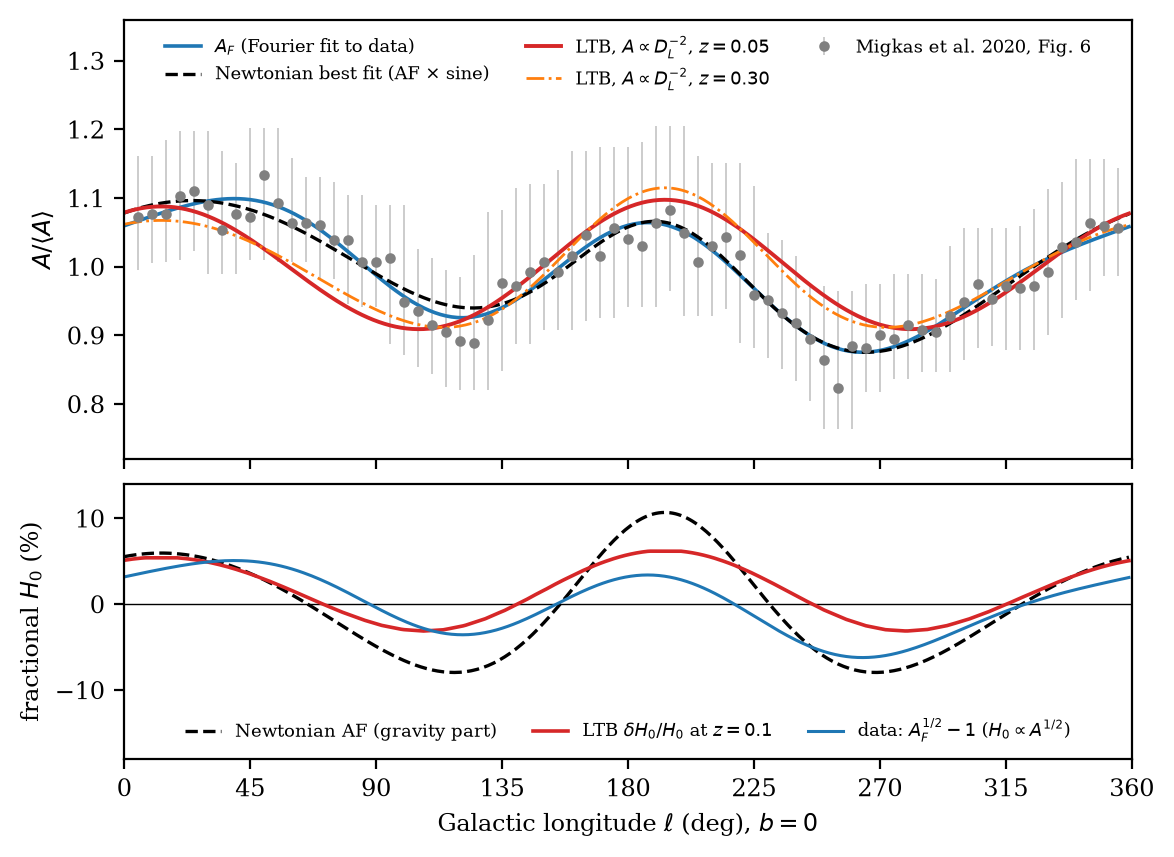
\includegraphics[width=0.6\textwidth]{fig_nearby.png}
\caption{Top: Migkas data, their Fourier fit $A_F$, your Newtonian best fit, and the LTB prediction $A\propto D_L^{-2}$ at $z=0.05$ and $0.3$. Bottom: fractional $H_0$ from the Newtonian AF, from the LTB, and from the data with $H_0\propto A^{1/2}$.}\label{fig:near}
\end{figure*}
\begin{table*}[t]\centering\small
\caption{Scan. Local $\Omega$, sky fraction with a density-defined LSS, nearby $m=2$ amplitude of $A$ at $z=0.1$, dipole-nulling $\beta$, boosted $|c_2|$, and $|c_2|/A_{m2}$. Above the rule: your pure CoE-mass family; below: open background plus lump at your $D$ and $L$.}\label{tab:scan}
\begin{tabular}{@{}lcccccc@{}}\toprule
Model & $\Omega_{\rm loc}$ & sky fraction & $A_{m2}$ & $\beta$ & $|c_2|$ & $|c_2|/A_{m2}$\\\midrule
\tabinput{tab_scan.tex}\bottomrule
\end{tabular}\end{table*}
\begin{table}[!t]\centering\footnotesize
\caption{Fourier amplitudes of $A(\ell)$ at $b=0$ (each normalised to its mean), the longitude of the $m=2$ maximum, and the correlation $r$ with the Migkas points, and the ratio of each curve $X$ on the CoE side to the anti-CoE side. The last row is $1+\delta H_0/H_0$.}\label{tab:near}
\setlength{\tabcolsep}{2pt}
\begin{tabular}{@{}lcccccc@{}}\toprule
Curve & $m=1$ & $m=2$ & $m=3$ & $\ell_{\max}$ & $r$ & $\frac{X(193^\circ)}{X(13^\circ)}$\\\midrule
\tabinput{tab_nearby.tex}\bottomrule
\end{tabular}\end{table}
\section{Nearby anisotropy in GR}
The LTB model produces a nearby Hubble anisotropy of the right size, shape and orientation (Table~\ref{tab:near}, Fig.~\ref{fig:near}). As in your Newtonian model it is almost pure $m=2$ and aligned with the CoE axis, and the LTB $\delta H_0/H_0$ follows the shape of your gravity term AF. Both put the fastest expansion along the axis ($H_r>H_\perp$, Table~\ref{tab:model}), as Eq.~(\ref{eq:tide}) requires for a positive net mass, so with $A\propto H_0^2$ the maximum of $A$ lies on the axis, where the data also have it. The GR amplitude is somewhat larger than the $m=2$ term of $A_F$, and the GR model has almost no $m=1$ or $m=3$, which in your fit come from the sine factor. Because the odd harmonics distinguish the CoE side from the anti-CoE side, we checked the angle convention explicitly. In your geometry $\theta=\ell-\ell_0$ and the source at $\theta=0$ lies farther from the CoE than Earth, so $\ell_0$ is the anti-CoE direction and the CoE lies at $\ell_0+180^\circ$; in the LTB code a ray launched at $\psi\to0$ moves to smaller shell radius, i.e.\ towards the CoE, and $\cos\psi=\cos(\ell-\ell_0-180^\circ)$ at $b=0$. With this convention both gravity terms are slightly larger on the CoE side, whereas the data and your sine-corrected fit are slightly larger on the anti-CoE side (last column of Table~\ref{tab:near}); that small odd part is supplied by your sine factor, not by gravity. The relativistic calculation therefore confirms the Newtonian conclusion for the dominant $m=2$ pattern.



\begin{figure}[t]\centering
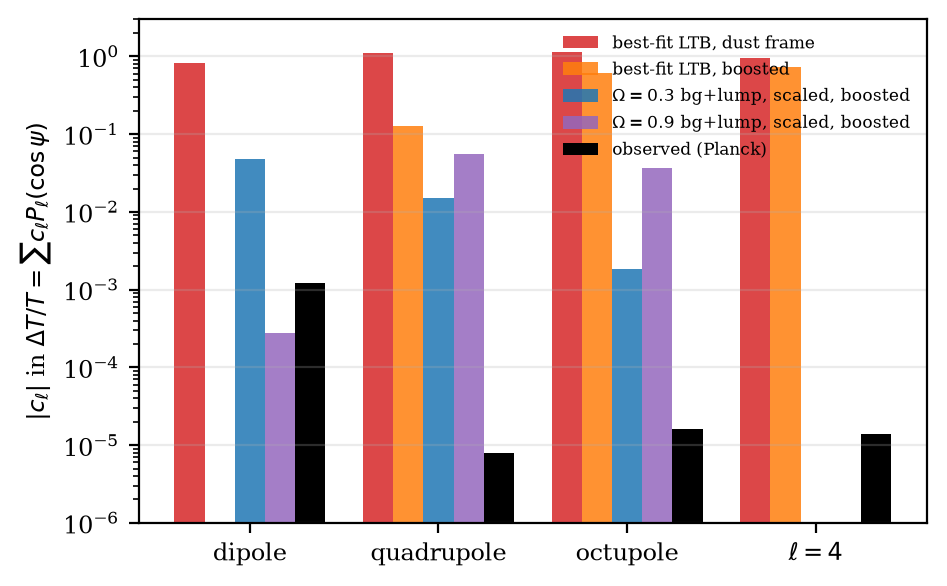
\includegraphics[width=\columnwidth]{fig_multipoles.png}
\caption{CMB multipoles of the models in Table~\ref{tab:mult} against the observed values. The boosted best-fit dipole is zero by construction.}\label{fig:mult}
\end{figure}



\section{CMB in pure dust: an open issue}
Figure~\ref{fig:dT}a and Table~\ref{tab:mult} give the result for the pure-dust best fit, in which the CMB temperature is set only by the gravitational stretch $1+z$ along each ray. The observer lies inside the gravitational radius of the enclosed mass but many scale lengths from the core, in a nearly empty region, and the density falls further outward. Rays within a cap around the CoE pass through the core, which was matter-dominated early on, and reach the recombination density. All other rays run back through almost empty, Milne-like space, where the density along the ray never reaches $\rho_{\rm rec}$. Under definition (b) most of the sky therefore has no last-scattering surface at all. Under definition (a) the stretch differs by order unity between the cap and the rest of the sky. The observed CMB dipole is kinematic \cite{Planck2013XXVII} and is not needed to support the model. Removing the model's intrinsic dipole with an observer boost would need a speed close to $c$, and the quadrupole and octupole would remain far above the observed level (Table~\ref{tab:mult}). How the CMB forms and propagates in the CoE picture, beyond pure dust with only gravitational redshift, is parked for a later stage.




\section{The pure-dust CMB with a background}
Table~\ref{tab:scan} gives a short scan. Within your family (a pure $e^{-r/L}$ CoE mass) lowering $M$, raising $D$ or lowering $D/L$ never gives a full-sky LSS, because a finite lump in otherwise empty space always leaves outward rays in vacuum, and a bang-time gradient only adds decaying modes \cite{Clarkson2011}. In pure dust, a last-scattering surface on every sightline requires a homogeneous background, such as the baryons-only background of the companion supernova note. With a background the problem becomes linear. The boosted CMB quadrupole is then a fixed fraction of the nearby $m=2$ amplitude, independent of the lump mass, which is the Grishchuk--Zel'dovich behaviour \cite{GZ1978,Turner1991,Erickcek2008}: the shear that makes $H_0$ anisotropic nearby acts on the photons all the way to the LSS. A nearby amplitude matching the data therefore implies a quadrupole about three orders of magnitude above the observed one (Table~\ref{tab:mult}), and passing the quadrupole limit leaves a nearby anisotropy far too small to see. LTB void studies find the same behaviour for an off-centre observer \cite{Alnes2006,Foreman2010,Enqvist2008,Clarkson2012}.


These statements hold for pure dust with gravitational redshift only, and they set the questions for the later CMB stage.

\section{Conclusion}
The exact relativistic version of your toy model reproduces what the Newtonian model was built to explain. The nearby anisotropy has the amplitude, the $m=2$ shape and the axis of the Migkas signal, with the corrected sign $A\propto H_0^2$ putting the maximum on the CoE axis (Table~\ref{tab:near}), even though $2GM/c^2>D$. The shell theorem explains why. Only the net mass inside $D-R$ produces the pattern, uniform matter enclosing the visible sphere changes only the mean rate, and the net mass must be positive for the pattern to have its observed orientation. The model is gravity-only and always decelerating, and nothing in this calculation requires changing that.

The CMB results are kept as a record of what pure dust gives, not as a verdict. In that limit most sightlines never reach recombination density, and adding a background gives a quadrupole that scales with the nearby shear. The observed dipole is kinematic and not required by the model. The physics of the CMB in the CoE picture is parked for a later stage.

The main caveats are that the model is pure dust without radiation, that case B is one choice of $E(r)$, that the nearby comparison uses $b=0$ only, and that the ``scaled'' rows extrapolate linear results.


\small
\begin{thebibliography}{99}\setlength{\itemsep}{0pt}
\bibitem{Migkas2020} K.~Migkas et al., A\&A 636, A15 (2020).
\bibitem{Migkas2021} K.~Migkas et al., A\&A 649, A151 (2021).
\bibitem{Bondi1947} H.~Bondi, MNRAS 107, 410 (1947).
\bibitem{Bolejko2011} K.~Bolejko, M.-N.~C\'el\'erier, A.~Krasi\'nski, Class.\ Quantum Grav.\ 28, 164002 (2011).
\bibitem{Hellaby1985} C.~Hellaby, K.~Lake, ApJ 290, 381 (1985).
\bibitem{Alnes2006} H.~Alnes, M.~Amarzguioui, Phys.\ Rev.\ D 74, 103520 (2006).
\bibitem{Foreman2010} S.~Foreman, A.~Moss, J.~P.~Zibin, D.~Scott, Phys.\ Rev.\ D 82, 103532 (2010).
\bibitem{Planck2018I} Planck Collaboration, A\&A 641, A1 (2020).
\bibitem{Planck2018V} Planck Collaboration, A\&A 641, A5 (2020).
\bibitem{Planck2013XXVII} Planck Collaboration, A\&A 571, A27 (2014).
\bibitem{Clarkson2011} C.~Clarkson, M.~Regis, JCAP 02, 013 (2011).
\bibitem{GZ1978} L.~P.~Grishchuk, Ya.~B.~Zel'dovich, Sov.\ Astron.\ 22, 125 (1978).
\bibitem{Turner1991} M.~S.~Turner, Phys.\ Rev.\ D 44, 3737 (1991).
\bibitem{Erickcek2008} A.~L.~Erickcek, S.~M.~Carroll, M.~Kamionkowski, Phys.\ Rev.\ D 78, 083012 (2008).
\bibitem{Enqvist2008} K.~Enqvist, Gen.\ Rel.\ Grav.\ 40, 451 (2008).
\bibitem{Clarkson2012} C.~Clarkson, C.\ R.\ Physique 13, 682 (2012).
\end{thebibliography}
\end{document}